\subsection{Identity Validation and Security}
Although many different ideas were proposed in the related works, the idea of identity tokens ended up being selected as the primary method for authentication in our prototype. The identity token system was selected primarily for its simplicity in implementation on the Android platform. Identity tokens are plain Java objects that are serialized using built in functionality of the Java libraries, and are thus easy to integrate with servers that are written in Java\cite{fongen1}\cite{fongen2011federated}.

The primary theory behind the identity tokens of being plain Java objects with short lifespans is retained in the protocol, but several other changes are made due to specific needs and challenges of our scenario. First, the identity tokens are no longer entirely public objects readable by the world. Instead, they are treated as confidential information and encrypted whenever they are sent over the network. This change was made to minimize the possibility of any security risk that may be exposed by a request for an identity token. In our scenario, a request for an identity token must be accompanied by the name (or another unique identifier) of the injured party whose health records are being sought out. This is necessary to include in the request since the requester (the medical response team) may have no prior knowledge of the injured party and cannot seek out the correct domain to request an identity token from without additional communications.

Thus, the response from the trust server must contain not only the identity token, but also information on where the health record server is that contains the requested records. The information that someone is injured or otherwise needing medical assistance is a large unintentional privacy violation if it is left unencrypted\cite{4451065}. Since this information needs to be encrypted, the encryption of the identity token does not add any complexity to the communication --- in fact, communication can be simplified, as all communication is encrypted identically. In addition, once the decision is made to encrypt the tokens, the request and response information can be included in the same Java object as the token, further simplifying the implementation of the protocol.
%\begin{wrapfigure}{r}{.35\textwidth}
%\begin{center}
%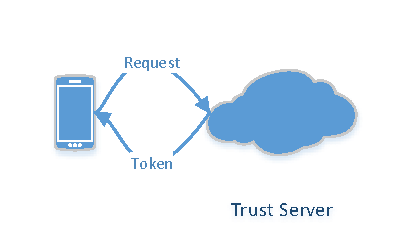
\includegraphics[scale=.75]{Drawing4.pdf}
%\caption{Request for a Token}
%\end{center}
%\end{wrapfigure}

As the identity token returned from the trust server now contains information about hospitals or health record servers that may be considered private, it is no longer wise to hand these out freely to any requester. Thus, the requesting party must verify their identity to the trust server. Table 1 reviews the properties of the identity token.

In our prototype, two-way SSL over HTTP is being used to satisfy the above needs. This handles the encryption as well as identity verification of the requester and the trust server in one step\cite{todd2003javaserver}. Correctly set up SSL should also check the revocation lists to ensure the requester has not lost their trust (for example, a certificate might be revoked after an employee no longer works at the hospital). In the prototype, Apache libraries\cite{apache} are combined with the standard Java libraries to set up the SSL connection. As SSL relies on trusted certificates distributed by a certificate authority, openSSL was used to generate and sign several certificates for all parties in the prototype\cite{manopenssl}.

\begin{center}
\begin{table}
  \begin{tabular}{ | l | l | }
    \hline
	 \multicolumn{2}{|l|}{Properties of Identity Token} \\ \hline
    userID & The userID that the requester is seeking records for. \\ \hline
    expiration & Tokens expire quickly so that they don't have to be checked for revocation. \\ \hline
    url & The URL of the Health Record Server that this token should be presented to. \\ \hline
    signature & The token is signed and hashed by the providing Trust Server. \\
    \hline
  \end{tabular}
  \caption{Properties of Identity Token}
\end{table}
\end{center}

\subsection{Trust Servers and Health Record Servers}

Of course, all the above statements rely on the existence of trust servers and health record servers that work as expected. In this case, the trust servers and health record servers were simulated by several servlets running in the Tomcat servlet container. Although these servlets were running on the same server, all communication between them was done over the network, as if they were running in separate environments.

As mentioned previously, a requester includes the name (or another more unique ID) of the individual whose health records are desired when requesting an identity token from a Trust Server. Because of the use of SSL, a Trust Server receiving a request can validate the identity of the requester. Sometimes a trust server will know exactly which health record server contains the request records, but oftentimes will have to discover this information and report it back to the requester. Ultimately, the returned product is an identity token that is signed by a Trust Server that is known to the Health Record Server holding the server. For example, if the records for ``Angela'' are held in Health Record Server A, then the requester needs to be returned an identity token signed by a Trust Server known to Health Record Server A.

Once a user has this identity token, it can then petition the Health Record Server for the records. Since the token is signed by a known Trust Server, the Health Record Server can trust that the requester has permission to access the records. The signature also ensures that the identity token was not modified. This prevents malicious users from impersonating an emergency health response team. This also prevents an emergency health response team from lying to the health record server and obtaining the records of a different person than reported to the trust server. The short expiration on the identity tokens also ensures that the requester has not had their trust revoked without having to consult a revocation list as is necessary in X.509\cite{fongen1}\cite{fongen2011federated}.

\begin{figure}[h]
\begin{center}
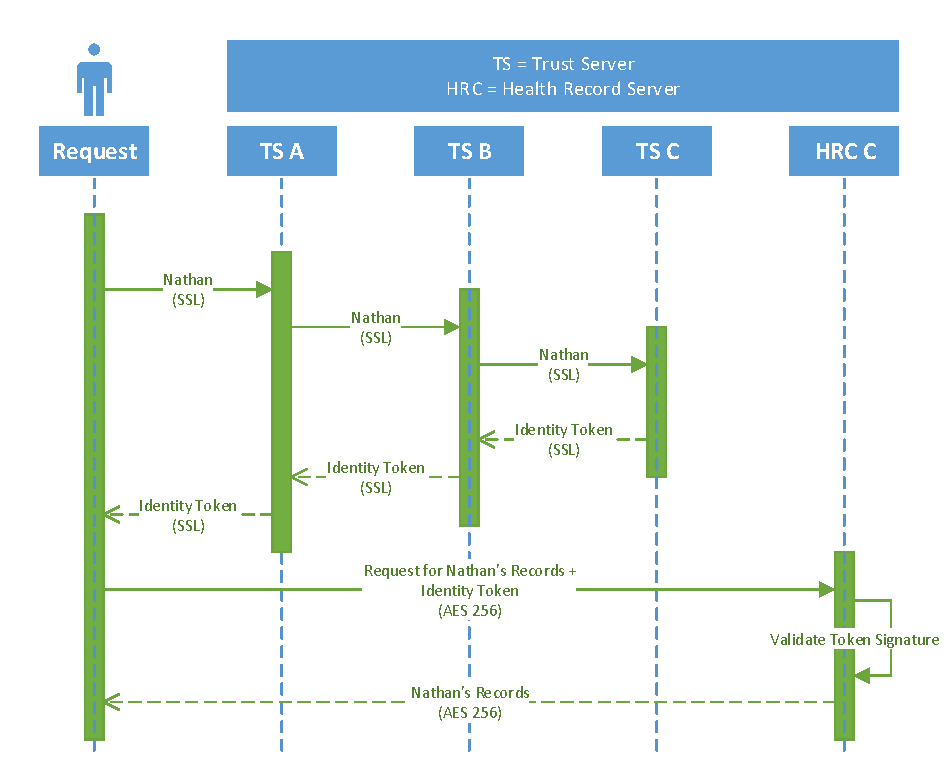
\includegraphics[scale=.75]{Drawing2.pdf}
\caption{Heath Record Retrieval Protocol}
\end{center}
\end{figure}

In the prototype, three Trust Servers and three Health Record Servers are simulated. The Trust Servers are named Trust Server A, Trust Server B, and Trust Server C. The Health Record Servers are named Health Record Server A, Health Record Server B, and Health Record C. Servers with like names are known to each other --- for example, Health Record Server A will trust identity tokens that are signed by Trust Server A. For the sake of testing, each Health Record Server contains two records. Server A contains the records of ``Angela'' and ``Rosendo''. Server B holds the records for ``Daniel'' and ``Marilyn''. Server C contains the records of ``Terry'' and ``Nathan''. Each Trust Server is aware what records their corresponding health record servers are responsible for, but does not know where any other records are held.

This means that if Trust Server A receives a request for the records of ``Nathan'', it does not know where those records are held --- only that they are not in Health Record Server A and that a token signed by Trust Server A will not be useful to the requester. Once a trust server determines that it cannot sign the token, it queries other nearby trust servers to try and retrieve the appropriately signed token for the requester. For the purposes of the prototype, Trust Server A knows of Trust Server B. Trust Server B knows of both Trust Servers A and C. Trust Server C knows only of Trust Server B. This means that a request for the health record of ``Nathan'' sent to Trust Server A will have to be forwarded to Trust Server B and finally C before a signed identity token can be returned to the requester. Since these requests are still carried out over SSL, Trust Server B is willing to trust someone trusted by Trust Server A, and so is willing to carry out its request for an identity token. In this way, a chain of trust is formed. The requester is finally returned the identity token signed by Trust Server C, as well as the URL (or other means of contact) of Health Record C, so that the requester can contact Health Record Server C directly for the records.

Upon receipt of the identity token signed by Trust Server C, Health Record Server C is then willing to send the records to the requester. As the requester and the Health Record Servers may not know each other and thus cannot use SSL, each communication should be encrypted using a symmetric key that is agreed upon beforehand. The prototype uses AES 256 to encrypt these communications. A symmetric key was chosen for the prototype as encryption using asymmetric keys is much costlier and slower. Figure 2 illustrates this entire process.

To handle most of the cryptography necessary in the prototype, the Bouncy Castle\cite{manbouncycastle} library was used to complement the built in Java functionality. Android features a version of Bouncy Castle build into the SDK, but it typically is not the latest version available. The prototype made use of some functionality only available in the newest release, but including the Bouncy Castle library in an Android project created package name conflict. To resolve this, a custom build of Bouncy Castle was created. This build simply moved everything to a unique package, as well as renamed the Bouncy Castle provider. This allowed the custom build to be registered from the Android project. As openSSL, Bouncy Castle, and Keytool (Java's bundled tool for dealing with keystores)\cite{mankeytool} operate using a variety of different formats, the open source tool Portecle\cite{manportecle} proved invaluable in converting between them.

\subsection{Performance}

The prototype seems to deliver the health records in a fairly timely fashion. Testing was done using a Motorola DRIOD 3 over a 3G connection. At the time of writing, both faster processors and faster cellular networks are fairly standard in mainstream consumer technology, so any time estimates obtained are reasonable. Figure 3 illustrates how including more Trust Server hops affected the round trip time from identity token request to identity token receipt.

\begin{figure}[h]
\begin{center}
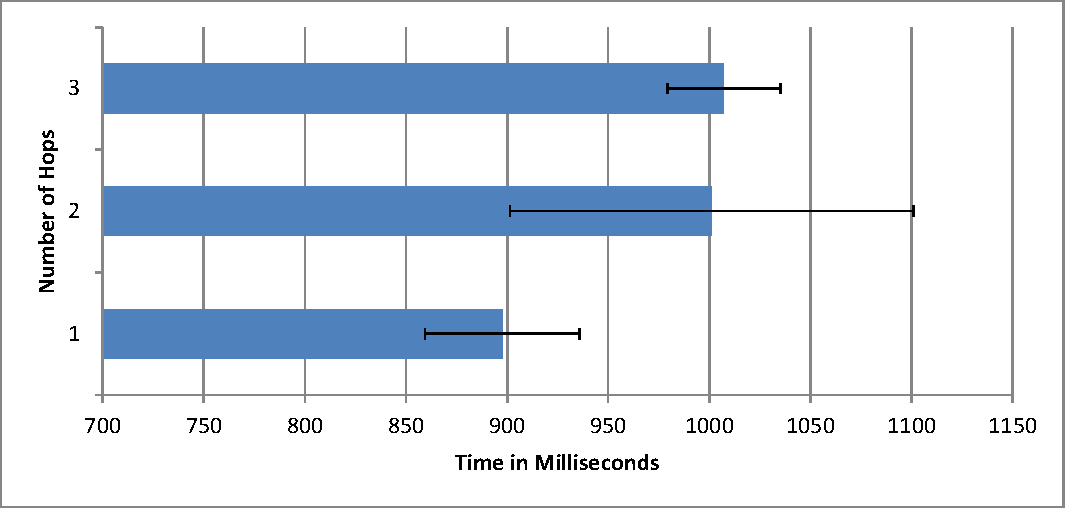
\includegraphics[scale=.65]{graph1.pdf}
\caption{Performance of Identity Token Fetching with 95\% Confidence Interval}
\end{center}
\end{figure}

The values in Figure 3 were obtained over an average of 10 requests. As can be seen, the difference is nearly nonexistent and can be attributed to network variance. These tests were performed with 3 Trust Servers in extremely close proximity, so the results are skewed somewhat. However, these numbers are still enough to see that the majority of the time spent fetching the identity token seems to be somewhat constant and tied to the single signature performed by the destination Trust Server.

Other computations that are performed by the phone are also completed fairly quickly, as illustrated in Figure 4.

\begin{figure}[h]
\begin{center}
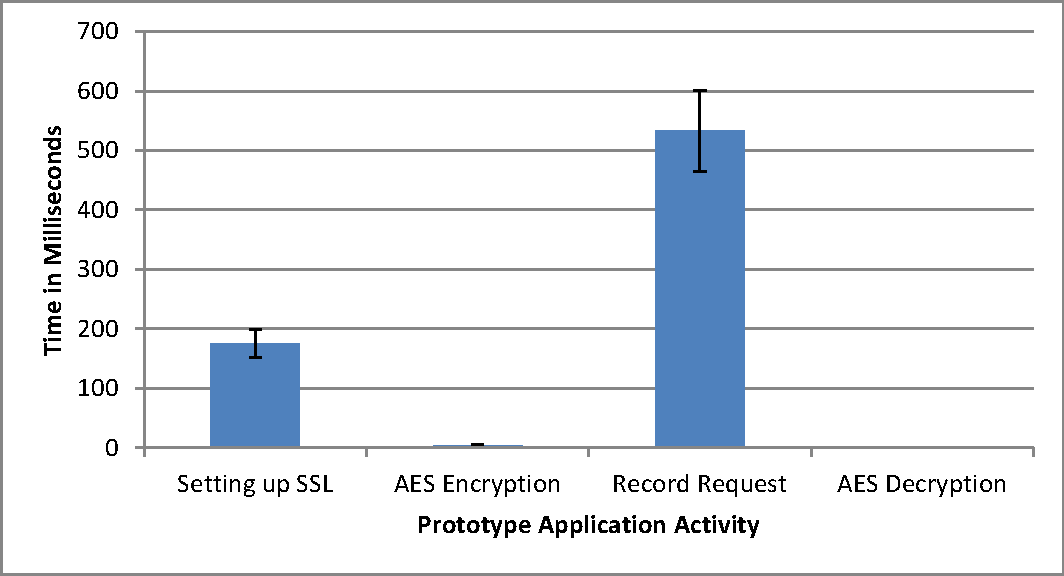
\includegraphics[scale=.65]{graph2.pdf}
\caption{Prototype Performance in Various Tasks with 95\% Confidence Interval}
\end{center}
\end{figure}

Concerns that the encryption/decryption of the health record requests would be too taxing for the phone's processor are quickly laid to rest. The largest bottleneck to performance seems to be the round trip delivery of the health records over the 3G network. This network call does not increase in complexity regardless of health record location, so this time is fairly constant and acceptable in performance.

The prototype seems fairly secure from a security standpoint. All communication is encrypted. There is room for the strengthening in the cryptographic techniques used, but should the appropriate precautions be taken, all communication can be considered reasonably secure. Considering the speed with which this is accomplished, the protocol seems like a reasonable success.